\documentclass{article}
\usepackage[french]{babel}
\usepackage[utf8]{inputenc}
\usepackage[T1]{fontenc}
\usepackage{microtype}
\usepackage{csquotes}
\usepackage{graphicx}
\usepackage[hidelinks]{hyperref}
\usepackage[backend=biber,style=ieee,sorting=nyt]{biblatex}
\usepackage[a4paper, left=3cm, right=3cm, top=3cm, bottom=3cm]{geometry}
\addbibresource{bibliography.bib}


\begin{document}

\begin{titlepage}
    \begin{center}
        {\Large \textbf{Université d'Évry Paris-Saclay}}\\[0.5cm]
        {\huge \textbf{État de l'art - Mémoire de Master}}\\[3cm]
        {\huge \textbf{Dans quelle mesure les technologies IoT des voitures peuvent-elles être adaptées pour répondre aux besoins spécifiques de la sécurité des motos sur les routes ? }}\\[1cm]
        \textbf{Année universitaire :} \\[0.5cm]
        {\Large \textbf{2024/2025}}\\[1cm]
                {\Large \textbf{Shana LEFEVRE}}\\[2cm]
                {\Large Maître d'apprentissage: \textbf{Clément LECLERCQ}}\\[0.5cm]
                {\Large Tutrice enseignante: \textbf{Farida ZEHRAOUI}}\\[2cm]
                \begin{figure}[h]
    \centering
    \includegraphics[width=0.7\textwidth]{images/logo_paris_saclay.png} 
\end{figure}
    \end{center}
\end{titlepage}

\tableofcontents % Table des matières
\newpage

\newpage
\section{Introduction}
%•	Présentation du sujet et de son importance.
\subsection{Contexte et enjeux}
%Abord IOT
L'IoT\footnote{Internet des objets} a révolutionné de nombreux aspects de notre société: la santé, de l'agriculture à l'industrie 4.0, en passant par les transports et les communications.
Les \textbf{technologies embarquées et connectées} désignent l’ensemble des systèmes électroniques intégrés aux véhicules (voitures et motos) permettant d’améliorer la sécurité, le confort et la connectivité. Ces technologies incluent :

%enjeux -> sécurité routière
L’accidentalité routière en France reste un enjeu majeur de sécurité publique, avec des milliers d’accidents chaque année causant des pertes humaines et matérielles importantes. Malgré les avancées en matière de prévention et de réglementation, les comportements à risque et les conditions de circulation continuent d’alimenter cette problématique.
En France, il y a environ 2,3 à 2,5 millions de motards\cite{actiEouteNbMotardFr}, ce qui représente 2\%  du trafic.
Le document\cite{la_securite_routiere_accidentalite_2024} fournit des informations et des statistiques sur les accidents de la route. Les données définitives datent du 31 mai 2024.

\begin{figure}[h]
    \centering
    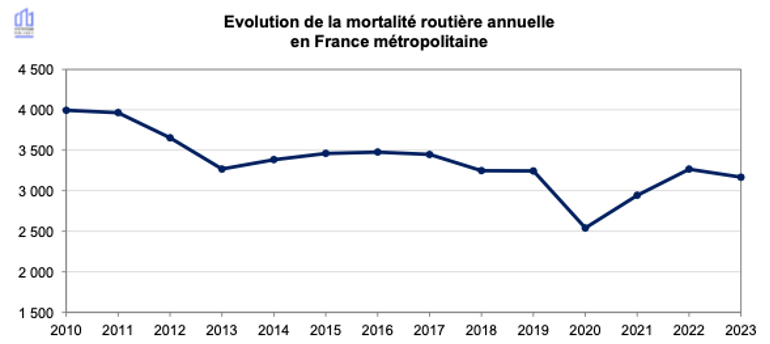
\includegraphics[width=0.7\textwidth]{images/evolution_mortalite_securite_routiere_france.png} 
    \caption{ONISR données relatives aux accidents corporels enregistrés par les forces de l'ordre en France métropolitaine.}
\end{figure}

Grâce au graphe précédent, on constate qu’il y a une diminution sensible du nombre d’accidents mortels sur la dernière décennie surtout entre 2011 et 2013. Différents paramètres expliquent cette évolution : nouvelles infrastructures routières, les dernières technologies de sécurité (casques, ABS…), les renforcements de la règlementation, mise en place de radars et nombreuses campagnes de sensibilisation… L’ensemble de ces éléments ont contribué à réduire la mortalité bien que chaque année, on enregistre, encore, autour de 3500 morts sur les routes tous véhicules confondus. 

\begin{figure}[h]
    \centering
    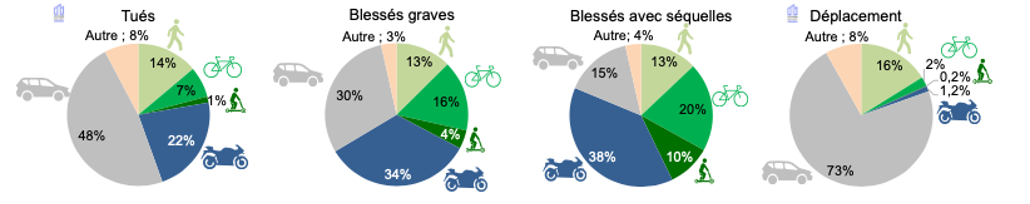
\includegraphics[width=0.7\textwidth]{images/camambert_accidents_differents_vehicules.png} 
    \caption{ONISR Données relatives aux accidents corporels enregistrés par les forces de l'ordre, en France métropolitaine.}
\end{figure}

En termes d’accidents corporels et de mortalité sur la route, les conducteurs de deux-roues sont les plus impactés. Le conducteur n’étant pas protégé par une carrosserie, il est plus vulnérable en cas d’accident. Le motard doit s’équiper de façon rigoureuse afin de limiter les blessures corporelles causées par le choc.


\subsection{Définitions et concepts clés}
%••	IoT (Internet des Objets) appliqué aux transports.
Qu'est-ce que l'IoT ?\\
L'IoT est un réseau d’objets physiques connectés à Internet qui sont capables de collecter et d’échanger des données en temps réel. Ces objets peuvent être des capteurs, des appareils domestiques intelligents, des équipements industriels, des véhicules et bien plus encore. Ils font face à des défis et des enjeux importants comme l'exposition aux menaces de cyberattaques, l'uniformité des systèmes pour leur bon fonctionnement, la consommation d'énergie et enfin, le respect aux droits privés. \\
• \textbf{Les capteurs et caméras} : détectent les obstacles, surveillent l’environnement et assistent à la conduite (ex. : radars, lidars, caméras 360°).\\
• \textbf{Les systèmes d’aide à la conduite (ADAS)} : aident le conducteur en régulant la vitesse, le freinage d’urgence ou le maintien de trajectoire.\\
• \textbf{Les modules de connectivité (4G, 5G, Wi-Fi, Bluetooth)} : permettent l’échange de données en temps réel entre le véhicule et d’autres systèmes, comme les infrastructures routières ou les smartphones.\\
• \textbf{Les plateformes de gestion des données} : traitent les informations collectées pour fournir des services comme la navigation intelligente, l’alerte trafic ou la maintenance prédictive.\\
Ces technologies sont essentielles pour le développement des véhicules intelligents et autonomes, ainsi que pour renforcer la sécurité des motards, souvent plus vulnérables sur la route.\\
\vspace{0.5cm}

Les \textbf{communications V2V (Vehicle-to-Vehicle) et V2I (Vehicle-to-Infrastructure)} font partie des technologies de transport intelligent (ITS)\footnote{infrastructure technology services} qui permettent aux véhicules et aux infrastructures routières d’échanger des informations en temps réel.


\newpage
\section{Les technologies IoT dans les voitures}

%introduction
Selon l’entreprise Objenious \cite{noauthor_revolution_2025}, l’Internet des Objets (IoT) constitue une révolution dans l’industrie automobile en rendant les véhicules plus intelligents et connectés. Depuis l’introduction de la norme européenne eCall en 2018, qui impose un système d’appel d’urgence automatique, les constructeurs ont intégré des technologies IoT pour développer des services innovants. Grâce aux réseaux haut débit comme la 4G et la 5G, les véhicules peuvent désormais collecter, envoyer et recevoir des données en temps réel, interagissant ainsi avec les infrastructures routières, les autres véhicules et les usagers.

Le marché mondial de l’IoT dans le secteur automobile, estimé à 115,37 milliards de dollars en 2022, devrait atteindre 975,66 milliards de dollars d’ici 2032, avec un taux de croissance annuel composé (TCAC) de 23,8 \% sur cette période \cite{noauthor_taille_2023}.

L’intégration des technologies IoT dans les véhicules permet une communication en temps réel entre les véhicules eux-mêmes, les infrastructures et d’autres dispositifs externes. Cette connectivité vise à améliorer la sécurité, l’efficacité et l’expérience de conduite. Les capteurs embarqués collectent et échangent des données sur les conditions de circulation, la météo, les performances du véhicule et le comportement du conducteur. Ces informations sont exploitées pour la maintenance prédictive, la navigation intelligente et l’optimisation des systèmes de conduite autonome.

Par ailleurs, la connectivité IoT facilite l’intégration des smartphones et autres appareils avec les véhicules, offrant ainsi des services tels que la surveillance à distance, le suivi des véhicules et des fonctionnalités d’infodivertissement personnalisées. Ces avancées technologiques redéfinissent le secteur automobile, ouvrant la voie à une mobilité plus sûre, plus intelligente et plus autonome.


\subsection{Systèmes de communication et d’échange de données}
%A développer
"Depuis longtemps une voiture collecte des données, ces données sont collectées via les capteurs et traitées par les calculateurs du véhicule." par Innovauto \cite{donnees_echange}.

%Données
Les différentes données émissent par un véhicule peuvent être \textbf{techniques} (ex: état de charge de la batterie, autonomie restante ...), \textbf{usage} (ex: trajet, style de conduite...) et \textbf{personnelles} (ex: titulaire de la carte grise, agenda du conducteur,...).
%cycle de vie de la donnée
Un véhicule autonome échange des données avec son environnement, et ces données suivent un cycle de vie comportant plusieurs étapes :

\begin{figure}[h]
    \centering
    \includegraphics[width=0.7\textwidth]{images/schéma_cycle_vie_donneées.png} 
    \caption{Cycle de vie de la donnée}
\end{figure}

Les étapes du cycle de vie des données doivent respecter le RGPD sans être spécifiquement adaptées à la pratique automobile. De plus, si des véhicules sont commercialisés, ils doivent se conformer aux normes de chaque pays, telles que le RGPD en Europe, le Cloud Act aux États-Unis, et le PIPL en Chine.

La connectivité des véhicules autonomes pose également des problèmes de sécurité, notamment la vulnérabilité aux attaques informatiques. Des questions se posent sur la manière de protéger ces systèmes contre de telles menaces. Comment peut-on sécuriser ces informations sensibles face aux cyberattaques ?

Nolwen LE GUENNEC\cite{le_gennec_machine_2023} souligne que le développement des voitures autonomes est ralenti par les difficultés informatiques, malgré les annonces d’Elon Musk. 


Les programmes informatiques consomment de l’énergie et l'impact environnemental de ces technologies doit être pris en compte.

Grâce à la technologie IoT, les véhicules peuvent échanger des données. Voici les 3 modes de fonctionnement des STI\footnote{Système de Transport Intelligent}.\\
- \textbf{Communication véhicule à véhicule (V2V)}:\\
Les véhicules équipés de l’IoT échangent des informations telles que leur vitesse et leur position. Cette communication permet de signaler des accidents ou des pannes, aidant les conducteurs à anticiper les problèmes de circulation et à se déplacer plus efficacement.\\
- \textbf{Communication véhicule à infrastructure (V2I)}:\\
Les véhicules connectés interagissent avec des éléments d’infrastructure routière comme les feux de circulation, les lampadaires et les caméras. 
L’analyse de ces données peut conduire à des ajustements tels que la modification des limites de vitesse ou la facilitation du passage des véhicules de secours, améliorant ainsi la sécurité routière pour tous les usagers.\\
- \textbf{Communication infrastructure au véhicule (V2I)}:\\
Les infrastructures routières transmettent des informations aux véhicules à proximité, permettant l’affichage en temps réel de données pertinentes pour les conducteurs.

\begin{figure}[h]
    \centering
    \includegraphics[width=0.7\textwidth]{images/schéma_systeme_communication_donnees.png} 
    \caption{Tableau du système de communication V2X d'Innovauto}
\end{figure}


\subsection{Capteurs et perception environnementale}
%•Caméras, LiDAR, radar, ultrasons.
%•Fusion de capteurs et algorithmes d’IA pour la reconnaissance des objets (motos incluses).
L'évolution des véhicules intelligents repose sur des systèmes de capteurs avancés de capteurs et de perception environnementale.
Ces technologies permettent aux véhicules de collecter, d'analyser et d'interpréter en temps réel leur environnement afin d'améliorer leur utilisation.
Les principaux capteurs utilisés sont les caméras, les radars, les lidars et les ultrasons.
Ces données permettent de :\\
- Détecter les pannes. \\
- Alerter les propriétaires en cas de dysfonctionnement. \\
- Optimiser la maintenance. \\
- Simplifier les procédures de réparation. \\
- Gerer les flottes de véhicules. \\

%Par exemple, Lormauto, un constructeur français spécialisé dans le rétrofit de véhicules, utilise la connectivité cellulaire 4G pour optimiser l’expérience utilisateur. Cette technologie permet de transmettre de grands volumes d’informations et de surveiller l’état de santé des véhicules et de leurs batteries en temps réel.

La perception de l'environnement consiste à analyser et interpréter les données fournies par les capteurs pour prendre des décisions en temps réel. La décision repose sur des algorithmes avancés d'IA\footnote{Intelligence Artificielle} qui permettent de reconnaître les objets, d'anticiper les comportements et de réagir en conséquence. Ces technologies sont essentielles pour la conduite autonome et la sécurité des usagers de la route, y compris les motards.
Pour cela, il faut combiner plusieurs informations:\\
- Détecter et classer les objets. \\
- Estimer leur vitesse et leur trajectoire. \\
- Anticiper les risques et les collisions. \\
- Améliorer la prise de décision.\\
Les avancées en intelligence artificielle, en connectivité (5G, V2X) et en traitement des données continueront d’améliorer la perception environnementale des véhicules, ouvrant ainsi la voie à une mobilité plus sûre, plus fluide et plus autonome. 

\subsection{Aide à la conduite et systèmes ADAS}
%•Détection des obstacles et freinage automatique.
%•Avertissements de collision et assistance au changement de voie.
Dans un monde où la sécurité routière est une priorité, les systèmes avancés d’aide à la conduite (ADAS\footnote{Advanced Driver Assistance System}) révolutionnent la manière dont les véhicules interagissent avec leur environnement, réduisant ainsi les risques d’accidents et améliorant l’expérience de conduite.
Selon le site du Gouvernement \cite{adas_gouv} "Ces technologies ouvrent la voie à des véhicules de plus en plus automatisés, mais ceux qui en sont équipés ne sont pas des véhicules dits « autonomes ». Les aides à la conduite ne remplacent pas le conducteur et ses obligations. Leur usage s’opère sous la surveillance permanente du conducteur, qui reste responsable de la tâche de conduite et de la maîtrise du véhicule."
\begin{figure}[h]
    \centering
    \includegraphics[width=0.7\textwidth]{images/ADAS_schéma.jpg} 
    \caption{Voiture embarquant des systèmes ADAS\cite{continental_adas}}
\end{figure}




\subsection{Analyse des données et prise de décision}
%•	Cloud computing et edge computing pour le traitement en temps réel.
%•	Machine Learning et IA pour l’anticipation des comportements routiers.
L'entreprise Valeo a conçu un radar Lidar « Scala ». D'après LeParisien \cite{le_parisien_radar_2019}, l'entreprise, en 2020 produit 200 000 exemplaires par an. Cette technologie permet à ce que la voiture conduit sans l'intervention d'un humain.


%yan Le Cun
Les recherches sur l'utulisation et l'interprétation des données recueillies par les capteurs sont au coeur des sujets depuis quelques années. Yann LeCun, précuseur du deep learning\footnote{L'apprentissage automatique.} nous présente l'interprétation et l'utilisation de données recueillies.
Ce graphe ci-dessous présente la relation entre l’écart de position d’une voiture sur la voie et l’angle du volant pour ramener la voiture au milieu. 

\begin{figure}[h]
    \centering
    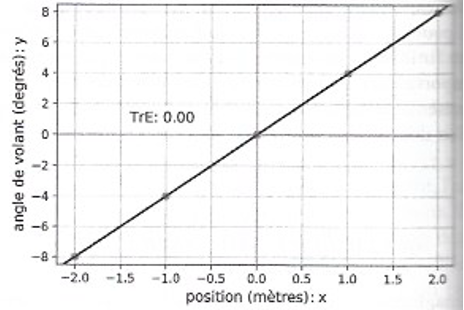
\includegraphics[width=0.7\textwidth]{images/graph1_yannLeCun.png} 
    \caption{Graphe page 88 du livre "Quand la machine apprend".}
\end{figure}

Par exemple, pour une déviation d’un mètre, il faudra incliner le volant de 4 degrés. 
Voici un nouvel exemple de graphique avec de nouvelles données d’entrée :

\begin{figure}[h]
    \centering
    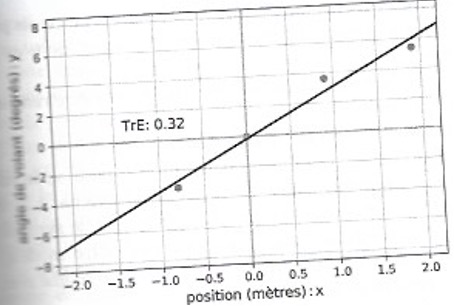
\includegraphics[width=0.7\textwidth]{images/graph2_yannLeCun.jpg} 
    \caption{Graphe page 88 du livre "Quand la machine apprend".}
\end{figure}

La pente passe par trois points sur quatre. Par conséquent, il faut trouver un compromis. On optera donc pour la solution où la droite passe au plus près des quatre points, comme modélisé précédemment. 




%Conclusion Technologie voitures IOT
En somme, l’IoT révolutionne l’industrie automobile en offrant des véhicules plus sûrs, plus efficaces et mieux entretenus, tout en ouvrant la voie à de nouvelles innovations dans le domaine de la mobilité.



%conférence
La mobilité autonome vise à garantir un confort et une fluidité optimaux, ce qui nécessite un système de surveillance pour mesurer diverses variables. Cela se fait principalement par l'utilisation de capteurs embarqués.
L'orientation et la direction de la roue jouent un rôle crucial, tout comme la mesure des longitudes et l'utilisation d'unités de mesure inertielle (IMU). La mesure de la vitesse latérale, en revanche, requiert des capteurs très coûteux d'après la conférence\cite{ahmed_ali_synthese_2024} de Sofiane AHMED ALI.
Pour réduire le nombre de capteurs nécessaires et, par conséquent, les coûts de développement, on peut utiliser des observateurs basés sur des modèles mathématiques pour déterminer les états du véhicule. Cette approche prometteuse présente toutefois des inconvénients, tels que la dynamique latérale du véhicule et les forces latérales agissant sur lui.
L'utilisation de capteurs visuels présente des défis supplémentaires. Ces capteurs peuvent allonger le processus de collecte de données et introduire des délais dans la transmission des images, ayant ainsi un impact majeur sur le système.




\newpage
\section{Les défis spécifiques liés à la sécurité des motos}

\subsection{Particularités des motos sur la route}
%•	Moins de visibilité et plus de vulnérabilité en cas d’accident.
%•	Dynamique de conduite différente des voitures (accélération rapide, inclinaison dans les virages).
Les motos présentent plusieurs particularités sur la route qui influencent leur sécurité et leur interaction avec les autres véhicules.
Une moto, c'est petit et ne possède que deux roues. Cela implique alors qu'elle est encore moins visible, surtout dans les angles morts d'un autre véhicule. Les motos sont agiles, possèdent une forte accélération et donc sûrement imprévisibles. Cela augmente le risque de collisions et les motos peuvent surprendre les autres usagers de la route. Sa configuration expose directement le conducteur deux-roues lors d'un accident par son manque de carrosserie. Les conditions météorologiques et la surface de la route jouent un rôle important dans l'adhérence des véhicules. Les conséquences sont beaucoup plus importantes pour un deux-roues car la chute est inévitable.
La puissance de la machine demande beaucoup d'anticipation et une conduite plus exigente face à tous les dangers.

\vspace{0.5cm} %conclusion
Ces particularités expliquent pourquoi la sécurité des motos sur la route est un enjeu majeur et nécessitent des adaptations spécifiques dans les systèmes de détection et d’assistance à la conduite. 

\subsection{Limitations des technologies IoT actuelles pour les motos}
%•	Problèmes de détection par les capteurs des voitures autonomes.
%	•	Communication insuffisante entre motos et véhicules connectés.
%	•	Difficultés d’adaptation des infrastructures intelligentes aux besoins des motards.


Le progrès côté deux-roues est très interessant et évolue.
La Verge TS Ultra est une moto électrique \cite{lenoir_cette_2024} haut de gamme intégrant des technologies avancées pour assurer une sécurité maximale à son pilote. Présentée lors du CES 2024, cette superbike est équipée du système Starmatter Vision, qui comprend six caméras et deux radars haute résolution, offrant une vision à 360 degrés de son environnement. Grâce à l’intelligence artificielle et au machine learning, la TS Ultra analyse en temps réel les risques potentiels et alerte le conducteur, notamment lors des changements de voie. Un écran agrandi sur le réservoir affiche des informations claires, comme la vue arrière lors de l’activation du clignotant. Côté performances, la moto dispose d’une batterie de 20,2 kWh alimentant un moteur de plus de 204 chevaux, permettant une accélération de 0 à 100 km/h en 2,5 secondes et une vitesse maximale limitée à 200 km/h. L’autonomie annoncée est de 375 km en conditions optimales, avec une recharge rapide possible en 25 minutes. La Verge TS Ultra est disponible à partir de 54 880 euros, avec des livraisons prévues pour le quatrième trimestre 2024.
Yamaha, en collaboration avec Netflix, a donné vie à la moto futuriste Y/AI \cite{texier_quand_2024} , initialement imaginée dans la série animée “Tokyo Override”. Cette moto, inspirée de la Yamaha YZR-M1 du MotoGP, présente un design avant-gardiste avec des roues sans rayons semi-transparentes émettant une lueur bleue en mouvement. Son moteur est dissimulé dans la structure reliant les roues, offrant une esthétique épurée. Les guidons, fixés sur les côtés des fourches avant et reliés par une arche, renforcent son allure futuriste. Ce prototype a été exposé au Motor Expo 2024 en Thaïlande, illustrant la vision de Yamaha sur l’intégration de l’intelligence artificielle dans les motos de demain.



%transition
Même si l'évolution et le progrès de cette technologie impressionnes et présente de bons résultats, elle de nombreuses limites et n'est pas encore au point. Quelles sont les limites ? Quels sont les dangers ?

\newpage
%limite de la tehnologie
\section{Les limites de la technologie}



%mentalité
D'après une étude réalisée par « The American Automobile Association (AAA) »\cite{consumer_skepticim} en Janvier 2022, il y a 85\% de la population interrogée exprime leur inquiétude, leur peur face à la technologie des voitures autonomes. En effet, cette technologie doit encore faire ses preuves à la population bien que des résultats soient prometteurs.

%les accidents
Les réseaux sociaux nous informent en temps réel des événements qui se déroulent dans notre pays ou à travers le monde. 
Récemment, j'ai lu un article\cite{journal_de_quebec_motocycliste_nodate} daté du jeudi 1er août 2024, relatant un incident survenu en avril dernier. Il s'agit d'un motocycliste de 28 ans, percuté par une voiture en conduite autonome, une Tesla Model S de 2022. Selon les données recueillies, la voiture aurait effectué une embardée après avoir perçu un bruit, ce qui a conduit à la collision. Le fabricant rappelle que ces véhicules ne sont pas entièrement autonomes et que le conducteur doit toujours être prêt à reprendre le contrôle en cas de problème. Selon l'Administration de la sécurité routière des États-Unis, 75 autres accidents impliquant des voitures autonomes ont été recensés. 
La semaine dernière, Elon Musk, PDG de Tesla, a déclaré que d'ici la fin de l'année, les systèmes de "conduite autonome" devraient être capables de fonctionner sans la supervision constante de son conducteur.











\newpage
\printbibliography
\end{document}

